\documentclass{article}
\usepackage{geometry}
\usepackage{graphicx}
\usepackage{amsmath}
\usepackage{algorithm}
\usepackage{algpseudocode}


\geometry{
a4paper,
right=20mm,
left=20mm,
top=20mm,
bottom=20mm,	
}

\begin{document}

\pagenumbering{gobble}

\begin{center}
\textbf{\huge Homework 1 : CS772} \\
\vspace{5pt}
\textit{\Large Jayant Agrawal}         14282
\end{center}

\section*{Problem 1}
\textbf{MLE} finds the parameter $\theta$ that maximises the log-likelihood($p(X|\theta)$)
$$\mathcal{L}(\theta) = log p(X|\theta) = log p(x_1, x_2 ...x_N | \theta)$$
Since the observations are i.i.d,
$$ p(x_1, x_2 ...x_n | \theta) = \prod_{n=1}^N p(x_n| \theta)$$
MLE Estimation,
$$\theta_{MLE} = argmax_{\theta} \mathcal{L}(\theta) = argmax_{\theta} \sum_{n=1}^N logp(x_n|\theta)$$
For poisson distribution,
$$\lambda_{MLE} = argmax_{\lambda} \sum_{n=1}^N logp(x_n|\lambda)$$
$$\lambda_{MLE} = argmax_{\lambda} \sum_{n=1}^N log\frac{\lambda^{x_n}e^{-\lambda}}{x_n!}$$
$$\lambda_{MLE} = argmax_{\lambda} \hspace{5pt} log\lambda\sum_{n=1}^Nx_n - N\lambda - \sum_{n=1}^Nlog(x_n!)$$
Setting the derivative to 0 to find $\lambda_{MLE}$,
$$\frac{1}{\lambda}\sum_{n=1}^Nx_n - N = 0$$
$$\mathbf{\lambda_{MLE}} = \frac{1}{N}\sum_{n=1}^Nx_n$$
\textbf{MAP} finds the parameter $\theta$ that maximises the log posterior probability($p(\theta|X)$)
$$\mathcal{L}(\theta) = log p(\theta|X) = log\frac{p(X|\theta)p(\theta)}{p(X)} $$
Since the observations are i.i.d, MAP estimation($\theta_{MAP}$) is given by,
$$\theta_{MAP} = argmax_{\theta} \mathcal{L}(\theta) = argmax_{\theta}\sum_{n=1}^N\log{p(x_n|\theta)}+ \log{p(\theta)} $$
For poisson distribution,
$$\lambda_{MAP} = argmax_{\lambda} \log{\lambda}\sum_{n=1}^Nx_n- N\lambda - \sum_{n=1}^Nlog(x_n!) + \log{\frac{\beta^\alpha}{\tau(\alpha)} \lambda^{\alpha-1} e^{-\beta\lambda}}$$
Setting the derivative to 0 to find $\lambda_{MAP}$,
$$\frac{1}{\lambda}\sum_{n=1}^Nx_n - N + \frac{\alpha-1}{\lambda}- \beta= 0$$
$$\mathbf{\lambda_{MAP}} = \frac{\sum_{n=1}^Nx_n + \alpha-1}{N+\beta}$$
\textbf{Posterior} Distribution will be proportional to the product of likelihood and prior:
$$ p(\theta| X) \propto \prod_{n=1}^N p(x_n|\theta) p(\theta) $$
For poisson distribution,
$$p(\lambda|X) \propto \prod_{n=1}^N p(x_n|\lambda) p(\lambda)$$
$$p(\lambda|X) \propto \prod_{n=1}^N \frac{\lambda^{x_n}e^{-\lambda}}{x_n!} \frac{\beta^\alpha}{\tau(\alpha)} \lambda^{\alpha-1}e^{-\beta \lambda}$$
$$p(\lambda|X) \propto  \frac{1}{\prod_{n=1}^{N}x_n!} \lambda^{\alpha + \sum_{n=1}^Nx_n -1}e^{-\lambda(N+\beta)}$$
Note that this is also a Gamma Distribution as(the proportionality constant comes after integrating the marginal likelihood in the denominator in the original expression of the posterior over $\lambda$), 
$$p(\lambda|X) = \text{Gamma}(\alpha + \sum_{n=1}^Nx_n, \beta + N)$$
Clearly, MAP estimate can be written as weighted combination of the MLE estimate and the prior's mode as,
$$\frac{\sum_{n=1}^Nx_n + \alpha-1}{N+\beta} = a*\frac{1}{N}\sum_{n=1}^Nx_n + b*\frac{\alpha-1}{\beta}$$
where $a$ and $b$ are scalars whose values are,
$$a = \frac{N}{N+\beta}$$
$$b = \frac{\beta}{N+\beta}$$
Since, posterior is also a Gamma Distribution, its mean is given by $\frac{\alpha_{pos}}{\beta_{pos}}$, which is,
$$\text{Posterior's Mean} = \frac{\sum_{n=1}^{N}x_n+ \alpha}{N+\beta}$$ 
Thus, Posterior's mean can be written as a weighted combination of the MLE estimate and the prior's mean as,
$$\frac{\sum_{n=1}^Nx_n + \alpha}{N+\beta} = a*\frac{1}{N}\sum_{n=1}^Nx_n + b*\frac{\alpha}{\beta}$$
where $a$ and $b$ are scalars whose values are,
$$a = \frac{N}{N+\beta}$$
$$b = \frac{\beta}{N+\beta}$$
\section*{Problem 2}
The variance of the posterior predictive distribution \textbf{decreases}. Intuitively, this is because, as the number of training examples increases, the uncertainty in the model decreases as we now we have some extra information about the underlying distribution. Formally, this can be seen by analysing the difference between $\sigma^2_{N+1}(x_*)$ and $\sigma^2_{N}(x_*)$.
$$\sigma^2_{N+1}(x_*) - \sigma^2_{N}(x_*) = (\beta^{-1} + x_*^{T}\Sigma_{N+1}x_*) - (\beta^{-1} + x_*^{T}\Sigma_{N}x_*)$$
$$\sigma^2_{N+1}(x_*) - \sigma^2_{N}(x_*) = x_*^{T}(\Sigma_{N+1} - \Sigma_N)x_* $$
Let $\Sigma_N/\beta = M_N^{-1}$ 
$$\sigma^2_{N+1}(x_*) - \sigma^2_{N}(x_*) = \beta*x_*^{T}((M_{N}+x_{N+1}x_{N+1}^T)^{-1} - M_N^{-1})x_* $$
Since we only care about the sign of this,
$$\text{sgn}(\sigma^2_{N+1}(x_*) - \sigma^2_{N}(x_*)) = \text{sgn}((M_{N}+x_{N+1}x_{N+1}^T)^{-1} - M_N^{-1}) $$
Using the identity given in the problem statement, 
$$\text{sgn}(\sigma^2_{N+1}(x_*) - \sigma^2_{N}(x_*)) = \text{sgn}(-\frac{(M_N^{-1}x_{N+1})(x_{N+1}^{T} M_N^{-1})}{1+x_{N+1}^TM_N^{-1}x_{N+1}}) $$
Since $M_N = (\sum_{n=1}^{N}x_nx_{n+1}^T + \frac{\lambda}{\beta
}I)$, is a covariance matrix and thus positive semi-definite. Therefore, 
$$\text{sgn}(\sigma^2_{N+1}(x_*) - \sigma^2_{N}(x_*)) = -1 $$
This shows that $\sigma^2_{N+1}(x_*)$ is less than $\sigma^2_{N}(x_*)$, thus proving that the variance decreases on increasing the number of training examples.

\section*{Problem 3}
\textbf{Case 1: Real Valued} \\
A suitable distribution in this case will be the gaussian distribution. A gaussian distribution is defined by a mean and a variance. In our case, $p(x_{nd}|y_n=k)$ is,
$$p(x_{nd}|y_n=k) = N(\mu_{dk}, \Sigma_{dk})$$
\textbf{MLE} Estimate: \\ \\
Log Likelihood is given by:
$$\log{p(D|\theta)} =  \sum_{k=1}^K\sum_{n:y_n=k}p(x_n|\theta_k) + \sum_{n=1}^N\sum_{k=1}^K 1[y_n=k]\log{\pi_k}$$
where the variables have the same meaning as the slides. For gaussian, 
$$p(x_n|\theta_k) = \prod_{d=1}^Dp(x_{nd}|y_n=k)$$
$$p(x_n|\theta_k) = \prod_{d=1}^DN(\mu_{dk}, \Sigma_{dk})$$
Now, MLE can be done easily, plugging in Log Likelihood expression, differentiating, and equating to zero for $\mu_{dk}$, 
$$ \mu_{dk} = \frac{1}{N_k}\sum_{n:y_n=k}x_{nd} $$
$$ \Sigma_{dk} = \frac{1}{N_k}\sum_{n:y_n=k}(x_{nd}-\mu_{dk})^2$$
where $N_k$ is the number of points with $y_n=k$. Also, MLE estimate for $\pi_k$ is same as that shown in slides,
$$\pi_k = \frac{N_k}{N} $$
\textbf{Case 2:Binary Valued} \\
Bernoulli Distribution will be ideal in this case, since the features are binary valued. This is described by a parameter $p_{dk}$, as,
$$p(x_{nd}|y_n=k) = p_{dk}^{x_{nd}}(1-p_{dk})^{1-x_{nd}}$$
Log Likelihood in this case is given as:
$$\log{p(D|\theta)} =  \sum_{k=1}^K\sum_{n:y_n=k} [x_{nd}\log{p_{dk}} + (1-x_{nd})\log{1-p_{dk}}] + \sum_{n=1}^N\sum_{k=1}^K 1[y_n=k]\log{\pi_k}$$
Now, for MLE, differentiating and equating to zero for $p_{dk}$,
$$\sum_{n:y_n=k}[(\frac{x_{nd}}{p_{dk}} - \frac{1-x_{nd}}{1-p_{dk}})] = 0 $$
$$\sum_{n:y_n=k}[ (x_{nd}-p_{dk})] = 0 $$
$$ p_{dk} = \frac{1}{N_k} (\sum_{n:y_n=k} x_{nd}) $$
MLE Estimate for $\pi_k$ is same as for Case 1. \\ \\
\textbf{Case 3:Discrete Valued} \\
There can be two choices for this case: Multinoulli and Binomial. MLE estimate for Binomial Distribution is shown here, as the values are sequential integers from 1 to $V$. Binomial Distribution is defined by $p_{dk}$ as,
$$p(x_{nd}|p_{dk}) = {{V}\choose{x_{nd}}}p_{dk}^{x_{nd}}(1-p_{dk})^{V-x_{nd}} $$
Log Likelihood in this case is given as:
$$\log{p(D|\theta)} =  \sum_{k=1}^K\sum_{n:y_n=k} [\log{{{V}\choose{x_{nd}}}}+x_{nd}\log{p_{dk}} + (V-x_{nd})\log{(1-p_{dk})}] + \sum_{n=1}^N\sum_{k=1}^K 1[y_n=k]\log{\pi_k}$$
Now, for MLE, differentiating and equating to zero for $p_{dk}$,
$$\sum_{n:y_n=k}[ (\frac{x_{nd}}{p_{dk}} - \frac{V-x_{nd}}{1-p_{dk}})] = 0 $$
$$\sum_{n:y_n=k}[\sum_{d=1}^D (x_{nd}-Vp_{dk})] = 0 $$
$$ p_{dk} = \frac{1}{VN_k} (\sum_{n:y_n=k} x_{nd}) $$
MLE Estimate for $\pi_k$ is same in this case also. \\ \\
\section*{Problem 4}
\begin{figure}[h!]
\begin{center}
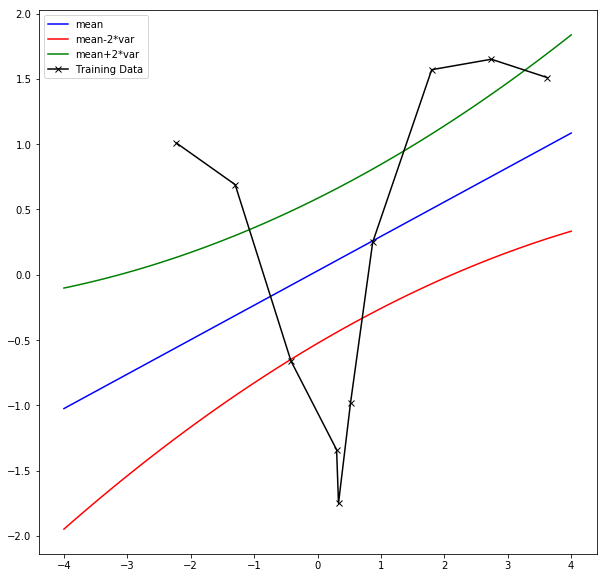
\includegraphics[scale=0.5]{one.png}
\label{one}
\caption{k=1}
\end{center}
\end{figure}

\begin{figure}[h!]
\begin{center}
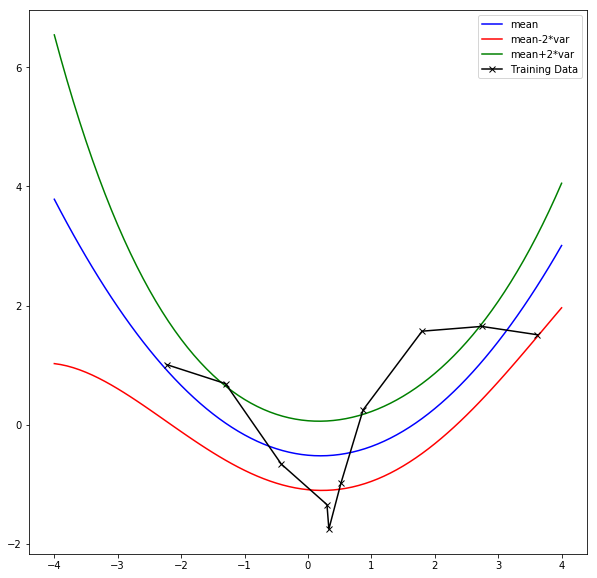
\includegraphics[scale=0.5]{two.png}
\label{two}
\caption{k=2}
\end{center}
\end{figure}

\begin{figure}[h!]
\begin{center}
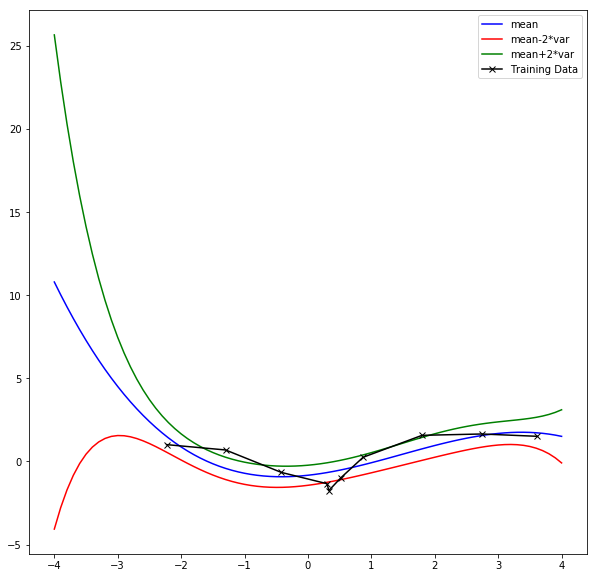
\includegraphics[scale=0.5]{three.png}
\label{three}
\caption{k=3}
\end{center}
\end{figure}

\textbf{Marginal Likelihood: } \\
\textit k = 1 : Marginal Likelihood = $8.90 \times 10^{-15}$ \\
\textit k = 2 : Marginal Likelihood = $1.28 \times 10^{-10}$ \\
\textit k = 3 : Marginal Likelihood = $2.57 \times 10^{-10}$ \\ \\
Since, marginal likelihood is maximum for $k=3$, thus this model explains the data "best". \\ \\
\textbf{Additional Training Input: }\\
Since, the models show highest variance around $x_* = -4$ (there are less number of training data points near $x = -4$), the extra data point should be near -4. \\
\textbf{Plots:} Mean of Posterior Predictive Distribution \\






\end{document}


